% Para utilizar este template siga o tutorial disponível em http://www.biblioteca.ufc.br/wp-content/uploads/2015/09/tutorial-sharelatex.pdf

%%%%%%%%%%%%%%%%%%%%%%%%%%%%%%%%%%%%%%%%%%%%%%%%%%%%%%%
%% Você deve criar uma conta no Overleaf. Depois,    %%
%% vá nas opções no canto esquerdo superior da tela  %%
%% e clique em "Copiar Projeto". Dê um novo nome pa- %%
%% ra o projeto.                                     %%
%%                                                   %%
%% Os principais desenvolvedores deste template são: %%
%%                                                   %%
%%            Ednardo Moreira Rodrigues              %%
%%       (Doutor em Engenharia Elétrica - UFC)       %%
%%(Coord. do Grupo de Astronomia da Seara da Ciência)%%
%%                      &                            %%
%%            Alan Batista de Oliveira               %%
%%           (Engenheiro Eletricista - UFC)          %%
%%                                                   %%
%% Consultoria Bibliotecária                         %%
%%                                                   %%
%%  Versão 2016 - ShareLaTeX:                        %% 
%%                                                   %%
%% - Francisco Edvander Pires Santos;                %%
%% - Juliana Soares Lima;                            %%
%% - Izabel Lima dos Santos;                         %%
%% - Kalline Yasmin Soares Feitosa;                  %%
%% - Eliene Maria Vieira de Moura.                   %%
%%                                                   %% 
%%  Versão 2019,2020 - Overleaf:                          %%
%%                                                   %%
%%  Biblioteca de Ciências Humanas:                  %%
%% - Francisco Edvander Pires Santos;                %%
%% - Juliana Soares Lima;                            %%
%% - Eliene Maria Vieira de Moura;                   %%
%% - Edmundo Moreira de Sousa Filho.                 %%
%%                                                   %%
%% Biblioteca da FEAAC:                              %%
%% - Izabel Lima dos Santos;                         %%
%% - Kalline Yasmin Soares Feitosa;                  %%
%% - Kleber Lima dos Santos.                         %%
%%                                                   %%
%%  Biblioteca do Curso de Física:                   %%
%% - Aline Rodrigues de Lima Mendes;                 %%
%% - Maria de Jesus Silva dos Santos.                %%
%%                                                   %%
%%  Biblioteca Central do Campus do Pici:            %%
%% - Raquel da Silva Nascimento.                     %%
%% - Felipe Ferreira da Silva                        %%
%%                                                   %%
%% Colaboradores                                     %%
%%                                                   %%
%% -Andrei Bosco Bezerra Torres                      %% 
%% (Professor - Sistemas e Mídias Digitais -         %%
%% Instituto Universidade Virtual - UFC)             %%
%% Tiago Alves Lima                                  %% 
%% (Aluno de Mestrado em Eng. Elétrica)              %%
%%                                                   %%
%% Grande parte do trabalho foi adaptado do template %%
%% da UECE elaborado por:                            %%
%% Thiago Nascimento  (UECE)                         %%
%% Project available on:                             %%
%% https://github.com/thiagodnf/uecetex2             %%
%%                                                   %%
%% "Dúvidas, esclarecimentos ou sugestões podem ser  %%
%% enviadas para o seguinte e-mail:                  %%
%%                                                   %%
%%             atendimentobch@ufc.br                 %%
%%                                                   %%
%% As últimas atualizações estão descritas no inicio %%
%% do arquivo "README.md".                           %%
%%                                                   %%
%%%%%%%%%%%%%%%%%%%%%%%%%%%%%%%%%%%%%%%%%%%%%%%%%%%%%%%

\documentclass[        
    a4paper,          % Tamanho da folha A4
    12pt,             % Tamanho da fonte 12pt
    chapter=TITLE,    % Todos os capitulos devem ter caixa alta
    section=Title,    % Todas as secoes devem ter caixa alta somente na primeira letra
    subsection=Title, % Todas as subsecoes devem ter caixa alta somente na primeira letra
    oneside,          % Usada para impressao em apenas uma face do papel
    english,          % Hifenizacoes em ingles
    spanish,          % Hifenizacoes em espanhol
    brazil,           % Ultimo idioma eh o idioma padrao do documento
    fleqn             % Comente esta linha se quiser centralizar as equacoes. Comente também a linha 65 abaixo
]{lib/abntex2}

\input{lib/preambulo}

\setlength{\mathindent}{0pt} %Complementa o alinhamento de equações para totalmente a esquerda.

%%%%%%%%%%%%%%%%%%%%%%%%%%%%%%%%%%%%%%%%%%%%%%%%%%%%%
%%                     ATENCAO                     %%
%%%%%%%%%%%%%%%%%%%%%%%%%%%%%%%%%%%%%%%%%%%%%%%%%%%%%
%  Qual e o nivel do trabalho academico que voce esta 
% escrevendo? Retire o simbolo "%" apenas de um dos 
% quatro topicos abaixo refente ao nível do seu traba
% -lho.

\trabalhoacademico{tccgraduacao}
%\trabalhoacademico{tccespecializacao}
%\trabalhoacademico{dissertacao}
%\trabalhoacademico{tese}

%%%%%%%%%%%%%%%%%%%%%%%%%%%%%%%%%%%%%%%%%%%%%%%%%%%%%

% Define se o trabalho e uma qualificacao
% Coloque 'nao' para versao final do trabalho

\ehqualificacao{nao}

% Remove as bordas vermelhas e verdes do PDF gerado
% Coloque 'sim' pare remover

\removerbordasdohyperlink{sim} 

% Adiciona a cor Azul a todos os hyperlinks

\cordohyperlink{nao}

%%%%%%%%%%%%%%%%%%%%%%%%%%%%%%%%%%%%%%%%%%%%%%%%%%%%%
%%         Informacao sobre a instituicao          %%
%%%%%%%%%%%%%%%%%%%%%%%%%%%%%%%%%%%%%%%%%%%%%%%%%%%%%

\ies{Universidade Federal do Ceará}
\iessigla{UFC}
\centro{Centro de Xxxxxxxx}
\departamento{Departamento de Xxxxxxxxx}

%%%%%%%%%%%%%%%%%%%%%%%%%%%%%%%%%%%%%%%%%%%%%%%%%%%%%
%%        Informacao para TCC de Graduacao         %%
%%%%%%%%%%%%%%%%%%%%%%%%%%%%%%%%%%%%%%%%%%%%%%%%%%%%%

\graduacaoem{Engenharia mecânica}
\habilitacao{bacharel} % Ou licenciado(a)

% AVISO: Caso necessario alterar o texto de apresenta-
% cao da Especializacao, ir a pasta "lib", arquivo 
% "ufctex.sty" na linha 502.


%%%%%%%%%%%%%%%%%%%%%%%%%%%%%%%%%%%%%%%%%%%%%%%%%%%%%
%%     Informacao para TCC de Especializacao       %%
%%%%%%%%%%%%%%%%%%%%%%%%%%%%%%%%%%%%%%%%%%%%%%%%%%%%%

\especializacaoem{Yyyyyyyyy}

% AVISO: Caso necessario alterar o texto de apresenta-
% cao da Especializacao, ir a pasta "lib", arquivo 
% "ufctex.sty" na linha 507.

%%%%%%%%%%%%%%%%%%%%%%%%%%%%%%%%%%%%%%%%%%%%%%%%%%%%%
%%         Informacao para Dissertacao             %%
%%%%%%%%%%%%%%%%%%%%%%%%%%%%%%%%%%%%%%%%%%%%%%%%%%%%%

\programamestrado{Programa de Pós-Graduação em Xxxxxxx}
\nomedomestrado{Mestrado Acadêmico em Xxxxxxx}
\mestreem{Engenharia Xxxxxx}
\areadeconcentracaomestrado{Engenharia Xxxxxx}

% AVISO: Caso necessario alterar o texto de apresenta-
% cao da dissertacao, ir a pasta "lib", arquivo 
% "ufctex.sty" na linha 511.

%%%%%%%%%%%%%%%%%%%%%%%%%%%%%%%%%%%%%%%%%%%%%%%%%%%%%
%%               Informação para Tese              %%
%%%%%%%%%%%%%%%%%%%%%%%%%%%%%%%%%%%%%%%%%%%%%%%%%%%%%

\programadoutorado{Programa de Pós-Graduação em Xxxxxx}
\nomedodoutorado{Doutorado em Xxxxxxx}
\doutorem{Engenharia Xxxxxx}
\areadeconcentracaodoutorado{Engenharia Xxxxxxx}

% AVISO: Caso necessario alterar o texto de apresenta-
% cao da tese, ir a pasta "lib", arquivo "ufctex.sty" 
% na linha 515.

%%%%%%%%%%%%%%%%%%%%%%%%%%%%%%%%%%%%%%%%%%%%%%%%%%%%%
%%      Informacoes relacionadas ao trabalho       %%
%%%%%%%%%%%%%%%%%%%%%%%%%%%%%%%%%%%%%%%%%%%%%%%%%%%%%

\autor{Paulo Cesar da Silva Junior}
\titulo{Contribuições para o entendimento da influência de variáveis na vibração de moinhos de rolos verticais, no processo de moagem do cimento com auxílio de Machine Learning.}
\data{2024}
\local{Fortaleza}

% Exemplo: \dataaprovacao{01 de Janeiro de 2012}
\dataaprovacao{}

%%%%%%%%%%%%%%%%%%%%%%%%%%%%%%%%%%%%%%%%%%%%%%%%%%%%%
%%           Informação sobre o Orientador         %%
%%%%%%%%%%%%%%%%%%%%%%%%%%%%%%%%%%%%%%%%%%%%%%%%%%%%%

\orientador{Profa. Dra. Rosineide Fernando da Paz}
\orientadories{Universidade Federal do Ceará (UFC)}
\orientadorcentro{Centro de Ciências e Tecnologia (CCT)}
\orientadorfeminino{nao} % Coloque 'sim' se for do sexo feminino

%%%%%%%%%%%%%%%%%%%%%%%%%%%%%%%%%%%%%%%%%%%%%%%%%%%%%
%%          Informação sobre o Coorientador        %%
%%%%%%%%%%%%%%%%%%%%%%%%%%%%%%%%%%%%%%%%%%%%%%%%%%%%%

% Deixe o nome do coorientador em branco para remover do documento

\coorientador{}
\coorientadories{Universidade Coorientador (SIGLA)}
\coorientadorcentro{Centro do Coorientador (SIGLA)}
\coorientadorfeminino{nao} % Coloque 'sim' se for do sexo feminino

%%%%%%%%%%%%%%%%%%%%%%%%%%%%%%%%%%%%%%%%%%%%%%%%%%%%%
%%              Informação sobre a banca           %%
%%%%%%%%%%%%%%%%%%%%%%%%%%%%%%%%%%%%%%%%%%%%%%%%%%%%%

% Atenção! Deixe em branco o nome do membro da banca para remover da folha de aprovacao

% Exemplo de uso:
% \membrodabancadois{Prof. Dr. Fulano de Tal}
% \membrodabancadoisies{Universidade Federal do Ceará - UFC}


\membrodabancadois{Prof. Dr. Xxxxxxx Xxxxxx Xxxxxxx}
\membrodabancadoiscentro{Faculdade de Filosofia Dom Aureliano Matos (FAFIDAM)}
\membrodabancadoisies{Universidade do Membro da Banca Dois (SIGLA)}
\membrodabancatres{Prof. Dr. Xxxxxxx Xxxxxx Xxxxxxx}
\membrodabancatrescentro{Centro de Ciências e Tecnologia (CCT)}
\membrodabancatresies{Universidade do Membro da Banca Três (SIGLA)}
\membrodabancaquatro{Prof. Dr. Xxxxxxx Xxxxxx Xxxxxxx}
\membrodabancaquatrocentro{Centro de Ciências e Tecnologia (CCT)}
\membrodabancaquatroies{Universidade do Membro da Banca Quatro (SIGLA)}
\membrodabancacinco{Prof. Dr. Xxxxxxx Xxxxxx Xxxxxxx}
\membrodabancacincocentro{Teste}
\membrodabancacincoies{Universidade do Membro da Banca Cinco (SIGLA)}
\membrodabancaseis{Prof. Dr. Xxxxxxx Xxxxxx Xxxxxxx}
\membrodabancaseiscentro{}
\membrodabancaseisies{Universidade do Membro da Banca Seis (SIGLA)}

\begin{document}	

	% Elementos pré-textuais
	\imprimircapa
	\imprimirfolhaderosto{}
	\imprimirfichacatalografica{1-pre-textuais/ficha-catalografica}
	%\imprimirerrata{elementos-pre-textuais/errata}
	\imprimirfolhadeaprovacao
	\imprimirdedicatoria{1-pre-textuais/dedicatoria}
	\imprimiragradecimentos{1-pre-textuais/agradecimentos}
	\imprimirepigrafe{1-pre-textuais/epigrafe}
	\imprimirresumo{1-pre-textuais/resumo}
	\imprimirabstract{1-pre-textuais/abstract}
	\renewcommand*\listfigurename{Lista de Figuras} %Se você comentar esta linha o título da lista fica: LISTA DE ILUSTRAÇÕES
	\imprimirlistadeilustracoes
	\imprimirlistadetabelas
	%\imprimirlistadequadros
	%\imprimirlistadealgoritmos
	%\imprimirlistadecodigosfonte
	\imprimirlistadeabreviaturasesiglas
	\imprimirlistadesimbolos{1-pre-textuais/lista-de-simbolos}   
	\imprimirsumario
	
	\setcounter{table}{0}% Deixe este comando antes da primeira tabela.
	
	%Elementos textuais
	\textual
	\chapter{Introdução}
\label{chap:introducao}

%Para começar a usar este \textit{template}, na plataforma \textit{ShareLatex}, vá nas opções (três barras vermelhas horizontais) no canto esquerdo superior da tela e clique em "Copiar Projeto" e dê um novo nome para o projeto. 

Para começar a utilizar este \textit{template}, siga o tutorial clicando no seguinte \textit{link}:
\url{http://www.biblioteca.ufc.br/images/arquivos/instrucoes_modelos/tutorial_sharelatex.pdf}


For further references see \href{http://www.sharelatex.com}{Something Linky} or go to the next url: \url{http://www.sharelatex.com} or open the next file \href{run:./file.txt}{File.txt}

Neste \textit{template}, o autor irá encontrar diversas instruções e exemplos dos recursos do uso do \LaTeX~na plataforma \textit{Overleaf}. O \LaTeX~foi desenvolvido, inicialmente, na década de 80, por Leslie Lamport e é utilizado amplamente na produção de textos matemáticos e científicos, devido a sua alta qualidade tipográfica \cite{goossens1994latex}. 

O \textit{Overleaf} é uma plataforma \textit{online} que pode ser acessado por meio de qualquer navegador de internet até mesmo de um \textit{smartphone}. Essa plataforma dispensa a instalação de aplicativos no computador para desenvolver trabalhos em \LaTeX. Também, não é necessário instalar \textit{packages}, ou seja, pacotes que permitem diferentes efeitos na formatação e no visual do trabalho. Todos os \textit{packages} que este \textit{template} utiliza são encontrados \textit{online}. 

Apresentam-se, também, neste modelo, algumas orientações de como desenvolver um trabalho acadêmico. Entretanto, este arquivo deve ser editado pelo autor de acordo com o seu trabalho sendo que a formatação já está de acordo com o aceito pela Universidade Federal do Ceará.  

A introdução, tem como finalidade, dar ao leitor uma visão concisa do tema investigado, ressaltando-se o assunto de forma delimitada, ou seja, enquadrando-o sob a perspectiva de uma área do conhecimento, de forma que fique evidente sobre o que se está investigando; a justificativa da escolha do tema; os objetivos do trabalho; o objeto de pesquisa que será investigado. Observe que não se divide a introdução em seções, mas a mesma informa como o trabalho ao todo está organizado.



%Testando o símbolo $\symE$

%\lipsum[5]  % Simulador de texto, ou seja, é um gerador de lero-lero.

%	\begin{alineas}
%		\item Lorem ipsum dolor sit amet, consectetur adipiscing elit. Nunc dictum sed tortor nec viverra.
%		\item Praesent vitae nulla varius, pulvinar quam at, dapibus nisi. Aenean in commodo tellus. Mauris molestie est sed justo malesuada, quis feugiat tellus venenatis.
%		\item Praesent quis erat eleifend, lacinia turpis in, tristique tellus. Nunc dictum sed tortor nec viverra.
%		\item Mauris facilisis odio eu ornare tempor. Nunc dictum sed tortor nec viverra.
%		\item Curabitur convallis odio at eros consequat pretium.
%	\end{alineas}
	

	

	\chapter{FUNDAMENTAÇÃO TEÓRICA}
\label{chap:fundamentacao-teorica}

Este capítulo apresenta os fundamentos teóricos necessários para compreender a aplicação de modelos de machine learning na predição de vibração em moinhos de rolos verticais. A fundamentação está estruturada de forma a contextualizar os equipamentos estudados, os fenômenos físicos envolvidos, as técnicas de aprendizado de máquina aplicáveis e as métricas utilizadas para comparação de desempenho dos modelos.

\section{Análise de Vibração em Equipamentos Rotativos}
\label{sec:analise-vibracao}

A análise de vibração constitui uma das técnicas fundamentais da manutenção preditiva, permitindo o monitoramento contínuo da condição mecânica de equipamentos rotativos \cite{rao2011mechanical}. A vibração em máquinas rotativas resulta da interação complexa entre forças desequilibradas, rigidez estrutural, amortecimento do sistema e excitações externas, manifestando-se como movimentos oscilatórios que podem ser medidos e analisados \cite{girdhar2004practical}.

Em equipamentos industriais, a vibração é caracterizada por sua amplitude, frequência e fase, sendo comumente expressa em unidades de velocidade (mm/s) ou aceleração (m/s²). A análise espectral da vibração permite identificar componentes específicas relacionadas a diferentes fontes de excitação, como desbalanceamento, desalinhamento, folgas mecânicas, defeitos em rolamentos e problemas de lubrificação \cite{mobley2002introduction}.

O desbalanceamento representa uma das principais causas de vibração em equipamentos rotativos, ocorrendo quando o centro de massa não coincide com o eixo de rotação. Este fenômeno gera forças centrífugas proporcionais ao quadrado da velocidade angular, resultando em vibração síncrona com a rotação do equipamento \cite{vance2010rotordynamics}. O desalinhamento entre eixos conectados produz componentes harmônicas características, particularmente na segunda harmônica da frequência de rotação, e pode acelerar significativamente o desgaste de acoplamentos e rolamentos.

A ressonância mecânica constitui outro aspecto crítico na análise de vibração, ocorrendo quando a frequência de excitação coincide com uma frequência natural do sistema. Nestas condições, pequenas forças podem produzir amplitudes de vibração extremamente elevadas, potencialmente causando danos estruturais graves \cite{inman2014engineering}. A identificação e evitação de condições de ressonância são fundamentais para o projeto e operação segura de equipamentos rotativos.

Os rolamentos representam componentes críticos em máquinas rotativas, sendo responsáveis por uma parcela significativa das falhas em equipamentos industriais. Defeitos em rolamentos produzem padrões de vibração característicos, com frequências específicas relacionadas à geometria do rolamento e à velocidade de rotação. A análise envelope e técnicas de demodulação são frequentemente empregadas para detecção precoce de defeitos em rolamentos \cite{randall2011rolling}.

A transmissão de vibração através da estrutura da máquina é influenciada pelas características dinâmicas do sistema, incluindo rigidez, amortecimento e massas envolvidas. Pontos de medição devem ser selecionados estrategicamente para capturar adequadamente os fenômenos de interesse, considerando caminhos de transmissão e frequências de ressonância estrutural \cite{scheffer2004machinery}.

Sistemas de monitoramento contínuo de vibração empregam acelerômetros ou sensores de velocidade instalados permanentemente nos equipamentos, permitindo acompanhamento em tempo real da condição mecânica. Estes sistemas frequentemente incorporam análise automatizada de tendências, detecção de alarmes baseada em limites pré-estabelecidos e capacidades de diagnóstico assistido por algoritmos de reconhecimento de padrões \cite{jardine2006review}.

A norma ISO 10816 estabelece critérios para avaliação de vibração em máquinas rotativas, definindo zonas de operação baseadas em amplitudes de velocidade de vibração. Zona A representa condição nova ou recém-reparada, Zona B indica operação satisfatória, Zona C sugere operação insatisfatória com necessidade de monitoramento intensivo, e Zona D requer ação corretiva imediata \cite{iso10816}.

\section{Moinhos de Rolos Verticais: Princípios e Falhas Características}
\label{sec:moinhos-rolos}

Os moinhos de rolos verticais constituem equipamentos fundamentais na indústria de processamento mineral, sendo amplamente utilizados na produção de cimento, beneficiamento de minérios e processamento de materiais industriais. Estes equipamentos operam através do princípio de moagem por pressão e cisalhamento, onde material alimentado no centro de uma mesa rotativa é submetido à ação de rolos pressurizados hidraulicamente \cite{austin1984introduction}.

A configuração típica de um moinho de rolos vertical compreende uma mesa rotativa horizontal, múltiplos rolos de moagem montados em braços articulados, sistema hidráulico de pressurização, separador de ar interno e sistema de exaustão. A mesa rotativa, acionada por motor elétrico através de redutor, distribui o material alimentado radialmente através da força centrífuga, formando uma camada de material entre a mesa e os rolos \cite{duda1985cement}.

O processo de moagem ocorre pela combinação de forças de compressão e cisalhamento aplicadas pelos rolos sobre o material depositado na mesa. A pressão hidráulica nos rolos, tipicamente variando entre 5-15 MPa, determina a intensidade da moagem e a finura do produto. O material moído é transportado pelo fluxo de ar ascendente até o separador interno, onde partículas finas são coletadas enquanto material grosso retorna à zona de moagem \cite{locher2006cement}.

A estabilidade operacional dos moinhos verticais depende criticamente da manutenção de uma camada uniforme de material na mesa de moagem. Flutuações na alimentação, variações nas características do material ou perturbações no fluxo de ar podem desestabilizar esta camada, resultando em vibrações excessivas e redução da eficiência de moagem \cite{hesse2004process}.

Falhas características em moinhos de rolos incluem desgaste excessivo das superfícies de moagem, problemas no sistema hidráulico de pressurização, desalinhamento de rolos, desgaste de mancais principais e falhas no sistema de vedação. O desgaste das placas de desgaste na mesa e nos rolos representa a principal causa de paradas programadas, exigindo substituição periódica baseada em critérios de desgaste pré-estabelecidos \cite{tromans1989mill}.

O sistema hidráulico de pressurização dos rolos constitui componente crítico para operação estável. Falhas em cilindros hidráulicos, vazamentos internos, problemas no acumulador de nitrogênio ou degradação do fluido hidráulico podem resultar em instabilidade na força de moagem, causando vibrações e redução da produtividade \cite{gearless2010mills}.

Vibrações excessivas em moinhos verticais podem originar-se de múltiplas causas: instabilidade da camada de moagem, desbalanceamento da mesa rotativa, problemas nos mancais principais, interferência entre rolos e mesa, ou excitações externas transmitidas através da estrutura de suporte. A identificação precisa da fonte de vibração requer análise sistemática combinando medições de vibração, análise espectral e correlação com parâmetros operacionais \cite{reichardt2004vertical}.

A manutenção preditiva em moinhos verticais emprega monitoramento contínuo de parâmetros operacionais incluindo vibração, temperatura de mancais, pressões hidráulicas, corrente do motor principal e características do produto moído. A integração destes parâmetros através de sistemas de monitoramento avançados permite detecção precoce de anomalias e otimização das estratégias de manutenção \cite{holderbank1993mill}.

\section{Machine Learning em Manutenção Preditiva}
\label{sec:ml-manutencao}

A manutenção preditiva baseada em machine learning representa uma evolução natural dos sistemas tradicionais de monitoramento de condição, oferecendo capacidades avançadas de reconhecimento de padrões, predição de falhas e otimização de estratégias de manutenção \cite{lee2014prognostics}. A aplicação de técnicas de aprendizado de máquina em dados de monitoramento permite identificar relações complexas entre variáveis operacionais e condição dos equipamentos, frequentemente imperceptíveis através de análise manual tradicional.

Os sistemas de manutenção preditiva tradicionais baseiam-se em análise de limites fixos e tendências de parâmetros individuais, oferecendo capacidade limitada para capturar interações multivariadas complexas. Machine learning supera estas limitações através de algoritmos capazes de processar simultaneamente múltiplas variáveis, identificar padrões não-lineares e adaptar-se automaticamente às características específicas dos equipamentos monitorados \cite{susto2015machine}.

Algoritmos supervisionados de machine learning requerem dados rotulados para treinamento, onde exemplos de condições normais e anômalas são utilizados para construir modelos de classificação ou regressão. Em aplicações de manutenção preditiva, estes rótulos podem representar condições de falha conhecidas, níveis de degradação ou tempo restante até falha. A qualidade e quantidade dos dados rotulados influenciam diretamente a performance dos modelos desenvolvidos \cite{carvalho2019systematic}.

Técnicas de aprendizado não-supervisionado são particularmente valiosas quando dados rotulados são escassos, permitindo detecção de anomalias baseada exclusivamente em padrões de operação normal. Algoritmos como clustering, análise de componentes principais e autoencoders podem identificar condições operacionais atípicas sem necessidade de exemplos prévios de falhas \cite{zhao2019machine}.

O processamento de dados temporais em manutenção preditiva apresenta desafios específicos relacionados à natureza sequencial das observações. Séries temporais de sensores contêm informações sobre tendências de degradação, padrões sazonais e correlações temporais que devem ser adequadamente capturadas pelos algoritmos de machine learning. Técnicas de feature engineering temporal, incluindo estatísticas móveis, transformadas espectrais e análise de autocorrelação, são frequentemente empregadas para extrair características relevantes dos dados temporais \cite{wang2019deep}.

A seleção de características (feature selection) constitui etapa crítica no desenvolvimento de modelos preditivos, especialmente quando lidando com datasets de alta dimensionalidade comuns em aplicações industriais. Técnicas de seleção baseadas em correlação, importância mutual e métodos embedded permitem identificar subconjuntos de variáveis mais relevantes para predição, reduzindo complexidade computacional e melhorando interpretabilidade dos modelos \cite{guyon2003introduction}.

A validação de modelos de machine learning em aplicações de manutenção preditiva deve considerar a natureza temporal dos dados, evitando vazamento de informação futuras (data leakage) durante treinamento. Técnicas de validação cruzada temporal, onde modelos são treinados em períodos passados e testados em períodos futuros, proporcionam estimativas mais realistas da performance em cenários operacionais reais \cite{cerqueira2020evaluating}.

A interpretabilidade dos modelos representa aspecto fundamental em aplicações industriais, onde engenheiros de manutenção necessitam compreender os fatores contribuintes para decisões automatizadas. Técnicas de explicabilidade como importância de características, valores SHAP e análise de sensibilidade permitem insights sobre o comportamento dos modelos e facilitam aceitação por parte dos usuários finais \cite{arrieta2020explainable}.

Sistemas de machine learning para manutenção preditiva devem incorporar capacidades de atualização incremental, permitindo adaptação contínua às condições operacionais em evolução. Algoritmos de online learning e transfer learning facilitam a incorporação de novos dados sem necessidade de retreinamento completo, mantendo relevância dos modelos ao longo do tempo \cite{khamassi2018discussion}.

A integração de modelos de machine learning em sistemas de manutenção existentes requer consideração cuidadosa de aspectos de latência, confiabilidade e manutenibilidade. Arquiteturas de edge computing permitem processamento local de dados de sensores, reduzindo latência e dependência de conectividade de rede, enquanto sistemas na nuvem oferecem capacidades computacionais superiores para modelos complexos \cite{shi2016edge}.

\section{Algoritmos de Machine Learning para Análise de Vibração}
\label{sec:algoritmos-ml}

A seleção apropriada de algoritmos de machine learning para análise de vibração depende das características específicas dos dados, objetivos de predição e requisitos operacionais. Diferentes famílias de algoritmos oferecem vantagens particulares para diferentes tipos de problemas de predição de vibração, desde regressão linear simples até ensemble methods complexos e redes neurais profundas \cite{zhao2019machine}.

Algoritmos de regressão linear representam a base fundamental para muitas aplicações de predição de vibração, oferecendo interpretabilidade superior e baixo custo computacional. A regressão linear assume relação linear entre variáveis preditoras e variável resposta, sendo particularmente efetiva quando esta suposição é válida. Regularização através de Ridge e Lasso regression permite lidar com multicolinearidade e seleção automática de características, respectivamente \cite{hastie2009elements}.

Árvores de decisão e métodos ensemble baseados em árvores, como Random Forest, oferecem capacidade de capturar relações não-lineares complexas entre variáveis de entrada e vibração. Random Forest combina múltiplas árvores de decisão através de bootstrap aggregating (bagging), reduzindo overfitting e fornecendo estimativas de incerteza através da variabilidade entre árvores individuais. A importância de características calculada pelo Random Forest fornece insights valiosos sobre variáveis mais relevantes para predição de vibração \cite{breiman2001random}.

Gradient boosting methods, incluindo XGBoost, LightGBM e CatBoost, representam estado da arte em muitas aplicações de machine learning estruturado. Estes algoritmos constroem modelos ensemble através de combinação sequencial de modelos fracos, onde cada modelo subsequente foca em corrigir erros dos modelos anteriores. XGBoost incorpora regularização avançada e otimizações computacionais que o tornam particularmente efetivo para dados tabulares típicos de aplicações industriais \cite{chen2016xgboost}.

Support Vector Machines (SVM) oferecem capacidades robustas para problemas de regressão através do conceito de margin maximization e uso de kernel functions para mapear dados para espaços de dimensionalidade superior. SVM com kernel RBF pode capturar relações não-lineares complexas, sendo particularmente efetivo em cenários com ruído e outliers. No entanto, o alto custo computacional pode limitar aplicabilidade para datasets grandes \cite{vapnik1998statistical}.

K-Nearest Neighbors (KNN) representa algoritmo baseado em instâncias que realiza predições baseando-se em similaridade com observações de treinamento. Para predição de vibração, KNN pode ser efetivo quando padrões locais são mais importantes que tendências globais. A seleção apropriada do número de vizinhos (k) e métricas de distância é crítica para performance do algoritmo \cite{cover1967nearest}.

Redes neurais artificiais oferecem capacidade universal de aproximação de funções, sendo capazes de modelar relações extremamente complexas entre variáveis de entrada e vibração. Arquiteturas feedforward multicamadas são comumente empregadas para problemas de regressão, enquanto redes recorrentes (LSTM, GRU) são particularmente adequadas para dados sequenciais temporais. O treinamento efetivo de redes neurais requer datasets grandes e consideração cuidadosa de hiperparâmetros para evitar overfitting \cite{goodfellow2016deep}.

Algoritmos robustos como Huber regression são especialmente valiosos em aplicações de vibração onde outliers são comuns devido a condições operacionais atípicas ou ruído de sensores. Huber regression combina propriedades de robustez dos estimadores L1 com eficiência dos estimadores L2, oferecendo performance estável na presença de observações atípicas \cite{huber1964robust}.

Ensemble methods que combinam predições de múltiplos algoritmos base podem oferecer performance superior através de redução de variância e bias. Voting regressors combinam predições através de média simples ou ponderada, enquanto stacking utiliza meta-learners para aprender combinações ótimas. A diversidade entre modelos base é fundamental para efetividade de métodos ensemble \cite{zhou2012ensemble}.

A seleção de hiperparâmetros representa aspecto crítico para otimização de performance de algoritmos de machine learning. Técnicas como grid search, random search e otimização Bayesiana permitem exploração sistemática do espaço de hiperparâmetros. Validação cruzada temporal deve ser empregada para evitar overfitting e fornecer estimativas realistas de performance em dados futuros \cite{bergstra2012random}.

Feature engineering específico para dados de vibração inclui extração de características no domínio da frequência através de FFT, análise de envelope para detecção de defeitos em rolamentos, estatísticas de ordem superior para capturar não-gaussianidade, e características temporais como RMS, kurtosis e crest factor. A qualidade das características extraídas influencia diretamente a performance dos algoritmos de machine learning \cite{lei2020applications}.

\section{Métricas de Avaliação para Modelos Comparativos}
\label{sec:metricas-avaliacao}

A avaliação sistemática de modelos de machine learning para predição de vibração requer utilização de métricas apropriadas que capturem diferentes aspectos de performance, incluindo precisão, robustez, calibração e eficiência computacional. A seleção de métricas deve alinhar-se com objetivos específicos da aplicação e considerar custos relativos de diferentes tipos de erros de predição \cite{botchkarev2018performance}.

O coeficiente de determinação (R²) representa métrica fundamental para avaliação de modelos de regressão, indicando a proporção da variância na variável dependente explicada pelo modelo. R² varia entre 0 e 1, onde valores próximos a 1 indicam alta capacidade explicativa. No entanto, R² pode ser inflado artificialmente pela inclusão de variáveis irrelevantes, sendo necessário considerar versões ajustadas que penalizam complexidade do modelo \cite{steel2013principles}.

Root Mean Square Error (RMSE) quantifica a magnitude típica dos erros de predição, sendo expressa nas mesmas unidades da variável dependente. RMSE penaliza mais fortemente erros grandes devido ao termo quadrático, sendo particularmente sensível a outliers. Esta métrica é valiosa quando erros grandes são especialmente indesejáveis, como em aplicações de segurança crítica \cite{willmott2005advantages}.

Mean Absolute Error (MAE) representa a magnitude média dos erros de predição, oferecendo interpretação mais direta que RMSE. MAE é menos sensível a outliers, fornecendo estimativa mais robusta da performance típica do modelo. A comparação entre RMSE e MAE pode revelar informações sobre a distribuição dos erros, onde RMSE significativamente maior que MAE indica presença de erros grandes ocasionais \cite{willmott2005advantages}.

Mean Absolute Percentage Error (MAPE) normaliza erros pela magnitude da variável dependente, permitindo comparação entre datasets com diferentes escalas. No entanto, MAPE apresenta limitações quando valores verdadeiros são próximos de zero, podendo resultar em valores infinitos ou instáveis. MAPE é particularmente útil para interpretação de resultados por stakeholders não-técnicos \cite{kim2016new}.

A análise de resíduos fornece insights importantes sobre adequação dos modelos através de exame de padrões sistemáticos nos erros de predição. Resíduos homoscedásticos e normalmente distribuídos indicam adequação das suposições do modelo, enquanto padrões sistemáticos podem sugerir necessidade de transformações ou modelos mais complexos. Testes de normalidade como Shapiro-Wilk e análise de heteroscedasticidade são ferramentas valiosas neste contexto \cite{montgomery2012introduction}.

Métricas de robustez avaliam estabilidade de performance dos modelos na presença de ruído, outliers ou mudanças nas condições operacionais. Técnicas como cross-validation com diferentes partições, análise de sensibilidade a perturbações nos dados e avaliação em subconjuntos específicos podem revelar vulnerabilidades dos modelos. A robustez é particularmente crítica em aplicações industriais onde condições operacionais podem variar significativamente \cite{huber2009robust}.

A eficiência computacional engloba tanto tempo de treinamento quanto tempo de inferência dos modelos. Tempo de treinamento é relevante para aplicações que requerem retreinamento frequente, enquanto tempo de inferência é crítico para sistemas de tempo real. Métricas como throughput (predições por segundo) e latência (tempo para uma predição) são particularmente relevantes para deployment em produção \cite{li2020federated}.

Métricas de calibração avaliam quão bem as estimativas de incerteza dos modelos correspondem à frequência real de erros. Modelos bem calibrados produzem intervalos de predição que contêm a proporção esperada de observações reais. Diagramas de calibração e estatísticas como Brier score permitem avaliação quantitativa da calibração \cite{guo2017calibration}.

A análise de overfitting através de comparação entre performance de treinamento e teste é fundamental para avaliação de generalização dos modelos. Diferenças significativas entre estas métricas indicam overfitting, sugerindo necessidade de regularização, redução de complexidade ou aumento da quantidade de dados de treinamento. Learning curves que mostram performance em função do tamanho do dataset podem orientar decisões sobre coleta adicional de dados \cite{domingos2012few}.

Testes estatísticos de significância, como testes t pareados ou testes não-paramétricos de Wilcoxon, permitem avaliação objetiva de diferenças de performance entre modelos. Estes testes consideram variabilidade estatística nas métricas de performance, fornecendo confiança estatística nas comparações. Correções para múltiplas comparações, como correção de Bonferroni, devem ser aplicadas quando comparando múltiplos modelos simultaneamente \cite{demsar2006statistical}.

\section{Trabalhos Relacionados e Estado da Arte}
\label{sec:trabalhos-relacionados}

A aplicação de machine learning para predição de vibração em equipamentos industriais tem sido objeto de crescente interesse na literatura científica, com contribuições significativas abrangendo desde técnicas básicas de regressão até arquiteturas avançadas de deep learning. Esta seção apresenta uma revisão dos principais trabalhos relacionados, destacando metodologias, resultados e limitações identificadas \cite{lei2020applications}.

\citeonline{zhang2018deep} desenvolveram uma arquitetura de rede neural convolucional (CNN) para classificação de falhas em rolamentos baseada em sinais de vibração. O estudo demonstrou superioridade das CNNs em comparação com métodos tradicionais de extração manual de características, alcançando acurácia superior a 99\% em dataset controlado. Limitações incluem avaliação restrita a condições laboratoriais e falta de validação em dados industriais reais com ruído e variabilidade operacional.

\citeonline{chen2019machine} compararam múltiplos algoritmos de machine learning (SVM, Random Forest, Neural Networks) para predição de vibração em turbinas eólicas, utilizando dados de 18 meses de operação. Random Forest apresentou melhor performance (R² = 0.87), superando SVM (R² = 0.82) e redes neurais (R² = 0.84). O estudo destacou a importância de feature engineering específico para o domínio, incluindo características espectrais e estatísticas de ordem superior.

\citeonline{wang2020predictive} propuseram framework integrado combinando análise de componentes principais (PCA) para redução de dimensionalidade com ensemble de algoritmos (Random Forest, XGBoost, Support Vector Regression) para predição de vibração em compressores centrífugos. A abordagem ensemble alcançou RMSE 15\% inferior aos modelos individuais, demonstrando benefícios da combinação de algoritmos complementares.

\citeonline{liu2019vibration} investigaram aplicação de Long Short-Term Memory (LSTM) networks para predição de vibração em mancais de máquinas rotativas, considerando dependências temporais nos dados. A rede LSTM superou modelos tradicionais de regressão (R² = 0.94 vs 0.78), especialmente em horizontes de predição de médio prazo (30-60 minutos). Limitações incluem alto custo computacional e necessidade de grandes quantidades de dados sequenciais.

\citeonline{zhao2019intelligent} desenvolveram sistema híbrido combinando Wavelet Transform para pré-processamento de sinais com ensemble de algoritmos (Gradient Boosting, Random Forest, Neural Networks) para diagnóstico de falhas em moinhos de rolos. O sistema alcançou acurácia de 95\% na classificação de condições operacionais, superando abordagens tradicionais baseadas em análise espectral manual.

\citeonline{kumar2020machine} realizaram estudo comparativo abrangente de algoritmos de machine learning para manutenção preditiva em equipamentos rotativos, avaliando 12 algoritmos diferentes em datasets de 5 tipos de equipamentos. XGBoost e Random Forest emergiram como algoritmos mais consistentes, apresentando boa performance em diferentes tipos de equipamentos e condições operacionais.

\citeonline{li2018fault} propuseram arquitetura de deep autoencoder para detecção de anomalias em vibração de equipamentos rotativos, focando em detecção não-supervisionada de condições anômalas. A abordagem demonstrou capacidade de detectar 92\% das falhas incipientes com taxa de falsos positivos inferior a 5\%, superando métodos tradicionais baseados em limites fixos.

\citeonline{ahmed2021comparative} conduziram análise comparativa de técnicas de feature selection para predição de vibração, avaliando métodos baseados em correlação, informação mutual e importância por árvores. Métodos embedded (baseados em Random Forest) apresentaram melhor trade-off entre redução de dimensionalidade e preservação de performance preditiva.

Lacunas identificadas na literatura incluem: (1) limitada validação em dados industriais reais com condições operacionais variáveis; (2) falta de comparações sistemáticas considerando múltiplas métricas de performance e eficiência computacional; (3) inadequada consideração de aspectos de interpretabilidade e explicabilidade dos modelos; (4) insuficiente análise de robustez a ruído e outliers comuns em ambientes industriais \cite{carvalho2019systematic}.

O presente trabalho contribui para o estado da arte através de: (1) comparação sistemática de múltiplos algoritmos em dados industriais reais de moinhos de rolos verticais; (2) avaliação abrangente considerando múltiplas métricas de performance, robustez e eficiência; (3) análise detalhada de feature importance e interpretabilidade dos modelos; (4) validação temporal rigorosa evitando data leakage; (5) consideração específica de características operacionais de moinhos verticais na indústria cimenteira \cite{susto2015machine}.
	\chapter{Metodologia}
\label{chap:metodologia}

% ir na literatura e falar sobre o modelo que será utilizado. Fazer de forma macro, sem entrar em detalhe nas fórmulas. ## DESCREVER A IDEIA

% Usar RandomForest e NeuralNetwork

% 1. Ideia da Regressão linear 
% 2. Ideia do RandomForest (usar em pt-br: Floresta aleatória)
% 3. Ideia do NeuralNetwork. (explicar só a de regressão) Vamos utilizar uma rede para regressão

O primeiro passo, que possibilitou o desenvolvimento do trabalho como um todo, foi o recebimento dos dados do processamento de cimento, na fábrica Apodi. \textbf{(... falar sobre os dados. Estrutura, colunas, etc...) (Falar sobre possíveis tratativas que foram necessárias ser feitas)}. Após a realização da curagem dos dados, pudemos partir para uma análise mais aprofundada, a fim de entender com o que estávamos trabalhando, através de uma análise exploratória dos dados. \textbf{(Falar sobre técnicas utilizadas na EDA... Mediana, média, boxplot, correlação, desvio padrão, etc...)}

Com o entendimento solidificado acerca do conjunto de dados, o próximo passo foi a aplicação dos modelos empregados que serão responsáveis pela predição do comportamento vibratório dos moinhos de rolos verticais.

\section{Inteligência artificial}

A inteligência artificial (IA) trata-se do campo que se concentra na pesquisa e no avanço de algoritmos que podem compreender e exibir comportamento inteligente, sem a intervenção humana no entendimento ou sem explicitamente dizer como responder a determinados estímulos \cite{Dinesh2024}. Os modelos de IA podem ser vistos nos smartphones, nos carros, nos bancos, nos hospitais, na aplicação da lei, nas organizações de seguros e em muitas outras aplicações \cite{Ali2023}.
 
\section{Regressão linear}

Nesse trabalho, a base geral de método preditivo aplicado foi a regressão linear. A qual, de acordo com \cite{HESAMIAN2024}, ajuda a identificar e quantificar as relações entre as variáveis, permitindo previsões e compreensão do impacto das variáveis independentes na variável dependente. 

Segundo \cite{Schneider2010}, a regressão linear é utilizada para estudar a relação linear entre uma variável dependente Y e uma ou mais variáveis independentes X. A variável dependente Y deve ser contínua, enquanto as variáveis independentes podem ser contínuas, binárias ou categóricas. O julgamento inicial de uma possível relação entre duas variáveis contínuas deve sempre ser feito com base em um gráfico de dispersão. Este tipo de gráfico mostrará se a relação é linear (figura \ref{fig:relacao-linear}) ou não linear (figura \ref{fig:relacao-exponencial}).

\pagebreak

 	\begin{figure}[h!] 
   	    \captionsetup{width=6cm}%Da mesma largura que a figura
		\Caption{\label{fig:relacao-linear} Gráfico de dispersão com relação linear.}
		\UFCfig{}{
			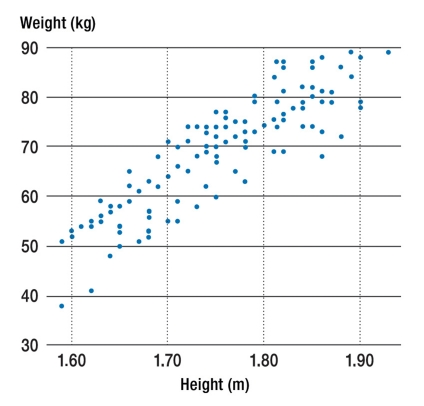
\includegraphics[width=6cm]{figuras/A scatter plot showing a linear relationship.jpg}
		}{
			\Fonte{\cite{Schneider2010}.}
		}	
	\end{figure}

  	\begin{figure}[h!] 
   	    \captionsetup{width=6cm}%Da mesma largura que a figura
		\Caption{\label{fig:relacao-exponencial} Gráfico de dispersão com relação exponencial.}
		\UFCfig{}{
			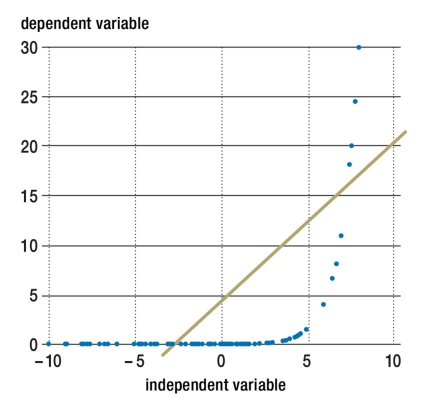
\includegraphics[width=6cm]{figuras/A scatter plot showing an exponential relationship.jpg}
		}{
			\Fonte{\cite{Schneider2010}.}
		}	
	\end{figure}

Quando temos uma relação linear, podemos dizer que as variáveis são correlacionadas em determinados graus. Porém, correlação não implica causalidade, e deve-se tomar cuidado para não tomar esse único indício como definitivo.

\pagebreak


\section{Floresta aleatória}

Falando de modelos de aprendizado de máquina, o primeiro utilizado baseia-se no princípio da floresta aleatória, a qual, de acordo com \cite{Wang2023}, é um método de aprendizado em conjunto que combina múltiplas árvores de decisão, usando \textit{bagging} (amostragem \textit{Bootstrap}) para reamostrar os dados originais e construir novos conjuntos de treinamento. Cada conjunto é usado para construir uma árvore de decisão, e a previsão final é feita pela média das saídas dessas árvores. Floresta aleatória é conhecida por sua escalabilidade e capacidade de lidar com dados de alta dimensão com menos parâmetros de otimização em comparação com outros métodos como Redes Neurais de Retropropagação (BPNN) e Regressão de Vetores de Suporte (SVR). Um esquema representativo de uma floresta aleatória é mostrado na figura \ref{fig:esquema-floresta-aleatoria}.

  	\begin{figure}[h!] 
   	    \captionsetup{width=12cm}%Da mesma largura que a figura
		\Caption{\label{fig:esquema-floresta-aleatoria} Esquema representativo de uma floresta aleatória.}
		\UFCfig{}{
			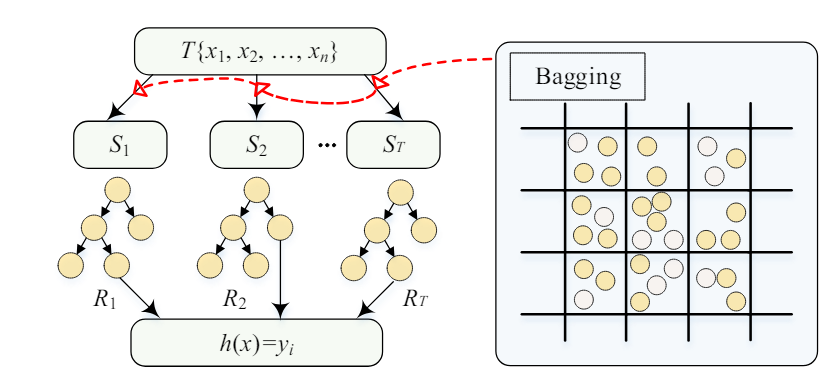
\includegraphics[width=12cm]{figuras/esquema-floresta-aleatoria.png}
		}{
			\Fonte{\cite{Wang2023}.}
		}	
	\end{figure}

 \subsection{Etapas de Implementação de uma floresta aleatória}

Primeiramente, a amostragem \textit{Bootstrap} é utilizada para reamostrar os dados originais, criando $T$ conjuntos de treinamento rotulados $S_1, S_2, \ldots, S_T$. Esses conjuntos de treinamento são então utilizados para construir árvores de regressão correspondentes $R_1, R_2, \ldots, R_T$. A cada nó, são amostrados aleatoriamente $T$ atributos de $M$, e o método de divisão ótima é aplicado utilizando o algoritmo CART, construindo o modelo $y = h(x)$. Para amostras de teste desconhecidas, calculam-se os valores previstos $R_1(X), R_2(X), \ldots, R_T(X)$ de cada árvore, e a média desses valores é usada como previsão final \cite{Wang2023}.

Devido à amostragem \textit{Bootstrap}, nem todos os dados originais são incluídos nos novos conjuntos de treinamento. Os dados excluídos formam a amostra \textit{Out-of-Bag (OOB)}, que é utilizada para validação cruzada embutida, avaliando o desempenho das árvores e estimando erros de generalização não tendenciosos \cite{Wang2023}.

 \subsection{Hiperparâmetros}

Os principais hiperparâmetros a serem ajustados são a profundidade das árvores e o número de preditores amostrados em cada nó. Árvores profundas tendem a \textit{overfitting}, enquanto árvores rasas podem sofrer de \textit{underfitting}. O número de preditores amostrados em cada nó afeta a precisão da previsão e precisa ser ajustado cuidadosamente para alcançar o melhor modelo \cite{Wang2023}.



\section{Redes neurais}

Segundo \cite{Kufel2023}, redes neurais artificiais se assemelham ao cérebro humano (Figura \ref{fig:diagrama-simplificado-neuoronio-humano}) e são compostas por múltiplos perceptrons ou ‘neurônios’ que processam e transmitem informações. Para entender seu funcionamento (Figura \ref{fig:esquema-nn}), começamos com a entrada de dados, como imagens, textos ou sons. Esses dados percorrem a rede, sendo processados por camadas sucessivas de neurônios até chegar à saída. Cada camada contém múltiplos neurônios que processam os dados de entrada.

\pagebreak

   	\begin{figure}[h!] 
   	    \captionsetup{width=12cm}%Da mesma largura que a figura
		\Caption{\label{fig:diagrama-simplificado-neuoronio-humano} Diagrama simplificado de um neurônio humano. 1—dendritos, local de entrada de sinal, 2—núcleo do neurônio, 3—zona de iniciação (onde o potencial de ação do neurônio é formado), 4—axônio, e 5—terminações axonais (que formam conexões com outras células e são os locais de saída de sinal), respectivamente.}
		\UFCfig{}{
			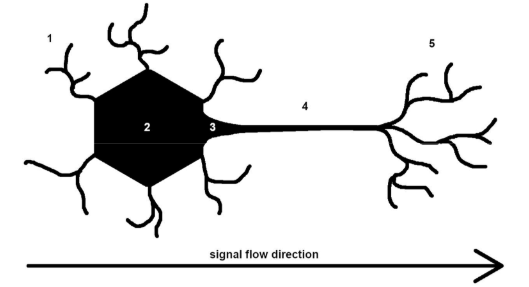
\includegraphics[width=12cm]{figuras/diagrama-simplificado-neuronio-humano.png}
		}{
			\Fonte{\cite{Kufel2023}.}
		}	
	\end{figure}

  	\begin{figure}[h!] 
   	    \captionsetup{width=12cm}%Da mesma largura que a figura
		\Caption{\label{fig:esquema-nn} Diagrama simplificado de um neurônio matemático. 1—entradas de sinal, 2—pesos, 3—somador, 4—ativador (função de ativação), e 5—saída de sinal, respectivamente.}
		\UFCfig{}{
			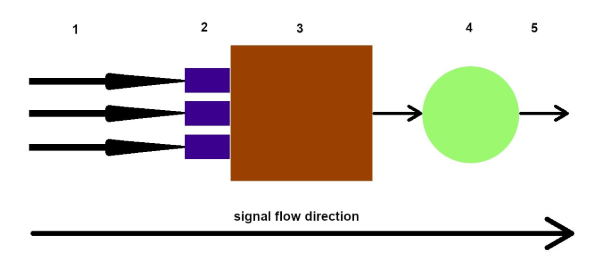
\includegraphics[width=12cm]{figuras/esquema-nn.png}
		}{
			\Fonte{\cite{Kufel2023}.}
		}	
	\end{figure}


 \pagebreak

Para treinar os perceptrons, os pesos são ajustados para minimizar a diferença entre a saída e o sinal esperado. A rede também aprende através do método da maior queda do gradiente, ajustando os comprimentos dos passos na direção oposta. Se o valor alvo em um novo ponto superar o ponto de partida, os passos são reduzidos até que o valor desejado seja alcançado (Figura \ref{fig:diagrama-nn}).

  	\begin{figure}[h!] 
   	    \captionsetup{width=10cm}%Da mesma largura que a figura
		\Caption{\label{fig:diagrama-nn} Diagrama simplificado da operação de uma rede neural.}
		\UFCfig{}{
			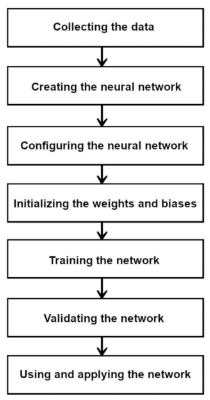
\includegraphics[width=10cm]{figuras/diagrama-nn.png}
		}{
			\Fonte{\cite{Kufel2023}.}
		}	
	\end{figure}

 \section{Long Short Term Memory (LSTM) Neural Network}

O modelo \textit{Long Short Term Memory (LSTM)} é uma evolução das Redes Neurais Recorrentes (RNN), que são compostas de várias camadas ocultas de neurônios em sequência, entre a camada de entrada e saída. O LSTM surgiu com o objetivo de resolver problemas típicos de RNN, como a perda de informações ao longo das camadas. As LSTMs são um tipo especial de RNN, capazes de aprender dependências de longo prazo e lembrar informações por períodos prolongados de tempo. A estrutura geral da LSTM também é de cadeia. Porém, em vez de uma única rede neural, existem quatro camadas com um método único de comunicação entre elas. A estrutura geral de uma LSTM pode ser observada na Figura \ref{fig:structure-of-a-lstm}.

  	\begin{figure}[h!] 
   	    \captionsetup{width=12cm}%Da mesma largura que a figura
		\Caption{\label{fig:structure-of-a-lstm} Estrutura de uma rede neural LSTM.}
		\UFCfig{}{
			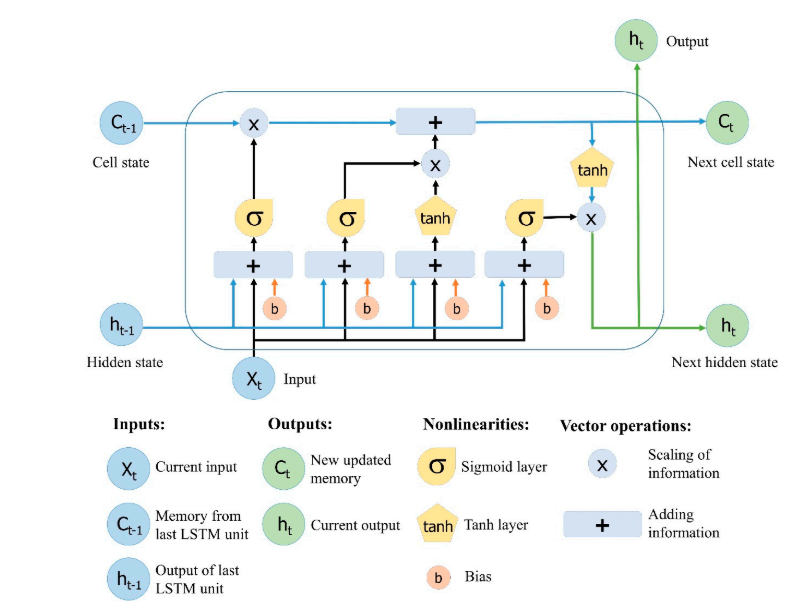
\includegraphics[width=12cm]{figuras/structure-of-a-lstm.png}
		}{
			\Fonte{\cite{Yan2016}.}
		}	
	\end{figure}

 % usar diagrama próprio

 começar pela exploração de dados
- separar variáveis que serão utilizadas, aquelas que acho que influenciam
- plotar gráficos de séries temporais de cada uma. Identificar ruídos e como removê-los

fazendo e escrevendo...
 

\section{Exemplo de alíneas}\label{sec:exemplo-de-algoritmos-e-figuras}

    Texto texto texto texto texto texto texto texto texto texto texto texto texto texto texto texto texto texto texto texto texto texto texto texto texto texto texto texto texto texto texto texto texto texto texto texto texto texto texto texto texto texto texto texto texto texto texto texto texto texto texto texto texto texto texto texto texto texto texto texto texto texto texto texto texto texto texto texto texto.

    %\begin{algorithm}[h!]
    %	\SetSpacedAlgorithm
    %	\caption{\label{exemplo-de-algoritmo}Como escrever algoritmos no \LaTeX2e}
    %	\Entrada{o proprio texto}
    %	\Saida{como escrever algoritmos com  Latex:}% \LaTeX2e }
    %	\Inicio{
    %		inicialização;
    %		\Repita{fim do texto}{
    %			leia o atual;
    %			\Se{entendeu}{
    %				vá para o proximo\;
    %				próximo se torna o atual;}
    %			\Senao{volte ao início da seção;}
    %		}
    %	}	
    %\end{algorithm}

    Texto texto texto texto texto texto texto texto texto texto texto.

    %\begin{algorithm}[H]
    %	\Entrada{o proprio texto}
    %	\Saida{como escrever algoritmos com \LaTeX2e }
    %	\Inicio{
    %		inicialização\;
    %		\Repita{fim do texto}{
    %			leia o atual\;
    %			\Se{entendeu}{
    %				vá para o próximo\;
    %				próximo se torna o atual\;}
    %			\Senao{volte ao início da seção\;}
    %		}
    %	}
    %	\caption{Exemplo de Algoritmo Versao 02}
    %\end{algorithm}

    %\begin{algorithm}
    %	\begin{algorithmic}
    %	\Entrada{o proprio texto}
    %	\Saida{como escrever algoritmos com \LaTeX2e }	
    %	\end{algorithmic}
    %\end{algorithm}

    Exemplo de alíneas com números:

    \begin{alineascomnumero}
	    \item Texto texto texto texto texto texto texto texto texto texto texto texto .
	    \item Texto texto texto texto texto texto texto texto texto texto texto texto .
	    \item Texto texto texto texto texto texto texto texto texto texto texto texto .
	    \item Texto texto texto texto texto texto texto texto texto texto texto texto .
	    \item Texto texto texto texto texto texto texto texto texto texto texto texto .
	    \item Texto texto texto texto texto texto texto texto texto texto texto texto .
    \end{alineascomnumero}

    Texto texto texto texto texto texto texto texto texto texto texto texto texto texto texto texto texto texto texto texto texto texto texto texto texto texto texto texto texto texto texto texto texto texto texto texto texto texto texto texto texto texto texto texto texto texto texto texto texto texto texto texto texto texto texto texto texto texto texto texto texto texto texto texto texto texto texto texto texto.

    Ou então figuras podem ser incorporadas de arquivos externos, como é o caso da \autoref{fig-grafico-1}. Se a figura que ser incluída se tratar de um diagrama, um gráfico ou uma ilustração que você mesmo produza, priorize o uso de imagens vetoriais no formato PDF. Com isso, o tamanho do arquivo final do trabalho será menor, e as imagens terão uma apresentação melhor, principalmente quando impressas, uma vez que imagens vetorias são perfeitamente escaláveis para qualquer dimensão. Nesse caso, se for utilizar o Microsoft Excel para produzir gráficos, ou o Microsoft Word para produzir ilustrações, exporte-os como PDF e os incorpore ao documento conforme o exemplo abaixo. No entanto, para manter a coerência no uso de software livre (já que você está usando LaTeX e abnTeX),  teste a ferramenta InkScape\index{InkScape}. ao CorelDraw\index{CorelDraw} ou ao Adobe Illustrator\index{Adobe! Illustrator}.  De todo modo, caso não seja possível  utilizar arquivos de imagens como PDF, utilize qualquer outro formato, como JPEG, GIF, BMP, etc.  Nesse caso, você pode tentar aprimorar as imagens incorporadas com o software livre \index{Gimp}Gimp. Ele é uma alternativa livre ao Adobe Photoshop\index{Adobe! Photoshop}.

\section{Usando fórmulas matemáticas}

Para escrever um símbolo matemático no texto, escreva símbolo entre cifrões, por exemplo, $\alpha$, $\beta$ e $\gamma$ são símbolo do alfabeto grego. Se você quiser inserir equações enumeradas, siga a estrutura de
\begin{equation}
    \label{eq:indices}
	k_{n+1} = n^2 + k_n^2 - k_{n-1}.
\end{equation}
Observe a pontuação, pois a equação faz parte da frase e do parágrafo. Como a equação faz parte da frase, não se utiliza o \textit{label} numérico \ref{eq:indices}. 

Quando for citar a Equação \ref{eq:indices} novamente no texto, utiliza-se o \textit{label} numérico. Repare que a palavra ``Equação'' foi escrita com ``E'' maiúsculo. 

Um exemplo de equações com frações é dado por
\begin{equation}
	\label{eq:fracao}
		\begin{aligned}
			x = a_0 + \cfrac{1}{a_1
				+ \cfrac{1}{a_2
					+ \cfrac{1}{a_3 + \cfrac{1}{a_4} } } }.
		\end{aligned}
	\end{equation}

Texto texto texto texto texto texto texto texto texto texto texto texto texto texto texto texto texto texto texto texto texto texto texto texto texto texto texto texto texto texto texto texto texto texto texto texto texto texto texto texto texto texto texto texto texto texto texto texto texto texto texto texto texto texto texto texto texto texto texto texto texto texto texto texto texto texto texto texto texto
	\begin{equation}
		\begin{aligned}
			k_{n+1} = n^2 + k_n^2 - k_{n-1}.
		\end{aligned}
	\end{equation}
	
Texto texto texto texto texto texto texto texto texto texto texto texto texto texto texto texto texto texto texto texto texto texto texto texto texto texto texto texto texto texto texto texto texto texto texto texto texto texto texto texto texto texto texto texto texto texto texto texto texto texto texto texto texto texto texto texto texto texto texto texto texto texto texto texto texto texto texto texto texto
	\begin{equation}
	\label{eq:trigo}
		\begin{aligned}
			\cos (2\theta) = \cos^2 \theta - \sin^2 \theta
		\end{aligned}.
	\end{equation}
	
Texto texto texto texto texto texto texto texto texto texto texto texto texto texto texto texto texto texto texto texto texto texto texto texto texto texto texto texto texto texto texto texto texto texto texto texto texto texto texto texto texto texto texto texto texto texto texto texto texto texto texto texto texto texto texto texto texto texto texto texto texto texto texto texto texto texto texto texto texto
	\begin{equation}
	\label{eq:matriz}
		\begin{aligned}
			A_{m,n} =
			\begin{pmatrix}
			a_{1,1} & a_{1,2} & \cdots & a_{1,n} \\
			a_{2,1} & a_{2,2} & \cdots & a_{2,n} \\
			\vdots  & \vdots  & \ddots & \vdots  \\
			a_{m,1} & a_{m,2} & \cdots & a_{m,n}
			\end{pmatrix}
		\end{aligned}.
	\end{equation}

Texto texto texto texto texto texto texto texto texto texto texto texto texto texto texto texto texto texto texto texto texto texto texto texto texto texto texto texto texto texto texto texto texto texto texto texto texto texto texto texto texto texto texto texto texto texto texto texto texto texto texto texto texto texto texto texto texto texto texto texto texto texto texto texto texto texto texto texto texto
	\begin{equation}
	\label{eq:sistema}
		\begin{aligned}
			f(n) = \left\{ 
			\begin{array}{l l}
			n/2 & \quad \text{if $n$ is even}\\
			-(n+1)/2 & \quad \text{if $n$ is odd}
			\end{array} \right.
		\end{aligned}.
	\end{equation}
Texto texto texto texto texto texto texto texto texto texto texto texto texto texto texto texto texto texto texto texto texto texto texto texto texto texto texto texto texto texto texto texto texto texto texto texto texto texto texto texto texto texto texto texto texto texto texto texto texto texto texto texto texto texto texto texto texto texto texto texto texto texto texto texto texto texto texto texto texto

%\section{Usando Algoritmos}

%\begin{algorithm}[h!]
%	\SetSpacedAlgorithm
%	\caption{\label{alg:algoritmo_de_colonica_de_formigas}Algoritmo de Otimização por Colônia de Formiga}
%	\Entrada{Entrada do Algoritmo}
%	\Saida{Saida do Algoritmo}
%	\Inicio{
%		Atribua os valores dos parâmetros\;
%		Inicialize as trilhas de feromônios\;
%		\Enqto{não atingir o critério de parada}{
%			\Para{cada formiga}{
%				Construa as Soluções\;
%			}
%			Aplique Busca Local (Opcional)\;
%			Atualize o Feromônio\;
%		}	
%	}		
%\end{algorithm}

\section{Usando código-fonte}

Um exemplo de código-fonte, ou código de programação encontra-se no Apendice \ref{ap:A}.

 
\section{Usando teoremas, proposições, etc}

 Texto texto texto texto texto texto texto texto texto texto texto texto texto texto texto texto texto texto texto texto texto texto texto texto texto.

\begin{teo}[Pitágoras]
	Em todo triângulo retângulo o quadrado do comprimento da
	hipotenusa é igual a soma dos quadrados dos comprimentos dos catetos. Usando o Apêndice \ref{ap:C}
\end{teo}


Texto texto texto texto texto texto texto texto texto texto texto texto texto texto texto.

\begin{teo}[Fermat]
	Não existem inteiros $n > 2$, e $x, y, z$ tais que $x^n + y^n = z$
\end{teo}

Texto texto texto texto texto texto texto texto texto texto texto texto texto texto texto.

\begin{prop}
	Para demonstrar o Teorema de Pitágoras...
\end{prop}

Texto texto texto texto texto texto texto texto texto texto texto texto texto texto texto.

\begin{exem}
	Este é um exemplo do uso do ambiente exem definido acima.
\end{exem}

Texto texto texto texto texto texto texto texto texto texto texto texto texto texto texto.


\begin{xdefinicao}
	Definimos o produto de ...
\end{xdefinicao}

Texto texto texto texto texto texto texto texto texto texto texto texto texto texto texto.

\section{Usando Questões} 

Um exemplo de questionário encontra-se no Apêndice \ref{ap:B}.

%Movido para o Apêndice


	\chapter{Resultados}
\label{chap:resultados}

Texto texto texto texto texto texto texto texto texto texto texto texto texto texto texto texto texto texto texto texto texto texto texto texto texto texto texto texto texto texto texto texto texto texto texto texto texto texto texto texto texto texto texto texto texto texto texto texto texto texto texto texto texto texto texto texto texto texto texto texto texto texto texto texto texto texto texto texto texto.

\section{Resultados do Experimento A}
\label{sec:resultados-do-experimento-a}

Procure deixar as figuras dos resultados o maior possível preenchendo a largura do texto do documento que possui $16~cm$.

\begin{figure}[h!]
        \captionsetup{width=16cm}
		\Caption{\label{fig:tensaoimpedanciahumana} Gráfico de tensão considerando a impedância humana}
		%\centering
		\UFCfig{}{
			\fbox{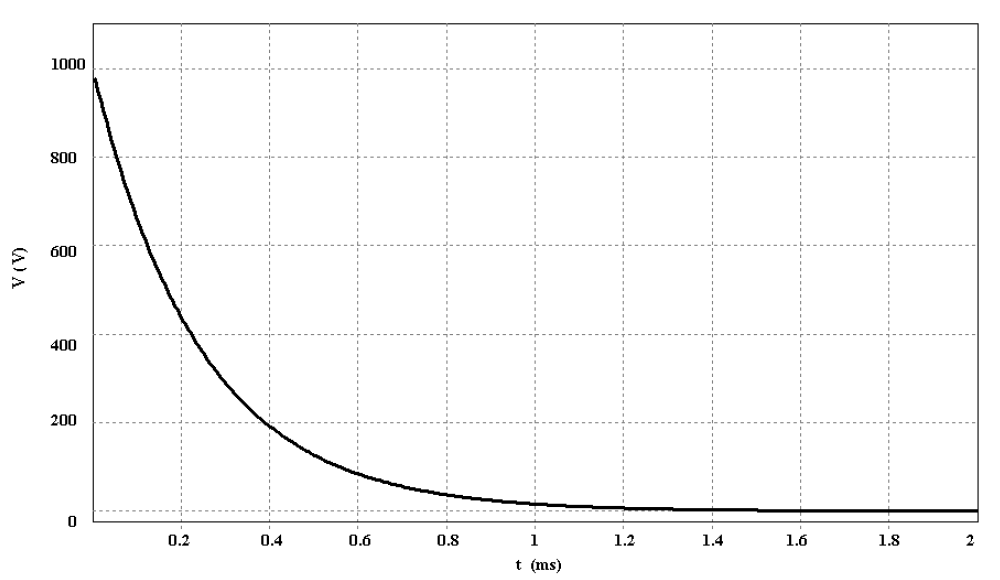
\includegraphics[width=16cm]{figuras/tensaoimpedanciahumana}}
		}{
			\Fonte{elaborado pelo autor (2016).}
		}	
\end{figure}

Texto texto texto texto texto texto texto texto texto texto texto texto texto texto texto texto texto texto texto texto texto texto texto texto texto texto texto texto texto texto texto texto texto texto texto texto texto texto texto texto texto texto texto texto texto texto texto texto texto texto texto texto texto texto texto texto texto texto texto texto texto texto texto texto texto texto texto texto texto.

\begin{figure}[h!]
	\captionsetup{width=16cm}
	\Caption{\label{fig-grafico-1}Produção anual das dissertações de mestrado e teses de doutorado entre os anos de 1990 e 2008}		
	\IBGEtab{}{
		\fbox{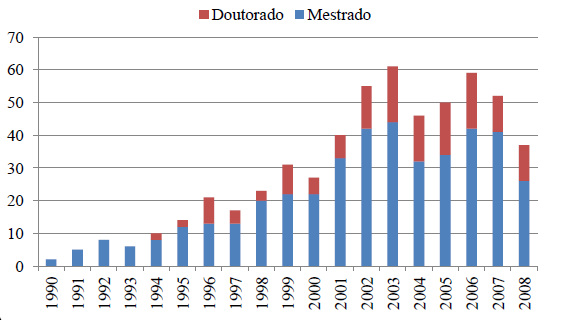
\includegraphics[width=16cm]{figuras/figura-3}}
	}{
	\Fonte{elaborado pelo autor (2016).}
}
\end{figure}

Texto texto texto texto texto texto texto texto texto texto texto texto texto texto.

Texto texto texto texto texto texto texto texto texto texto texto texto texto texto texto texto texto texto texto texto texto texto texto texto texto texto texto texto texto texto texto texto texto texto texto texto texto texto texto texto texto texto texto texto texto texto texto texto texto texto texto texto texto texto texto texto texto texto texto texto texto texto texto texto texto texto texto texto texto.

\section{Resultados do Experimento B}
\label{sec:resultados-do-experimento-b}

Referenciando a \autoref{tab:notas}. Texto texto texto texto texto texto texto texto texto texto texto texto texto texto texto texto texto texto texto texto texto texto texto texto texto texto texto texto texto texto texto texto.

\begin{table}[!ht]	
	%\centering
	\captionsetup{width=11.3cm}%ATENÇÃO: Ajuste a largura do título
	\Caption{\label{tab:notas} Notas dos participantes nas avaliações A, B e C}	
	\IBGEtab{}{
		\begin{tabular}{crrr}
			\toprule
			Identificação dos participantes & Avaliação A & Avaliação B &                        Avaliação C \\
			\midrule \midrule
			Participante 1 & 7 & 9 & 10\\
			Participante 2 & 8 & 2 & 1\\
			Participante 3 & 5 & 10 & 6 \\
			Participante 4 & 3 & 1 & 4\\
			Participante 5 & 2 & 4 & 1\\
			Participante 6 & 0 & 7 & 2\\
			\bottomrule
		\end{tabular}
	}{
	\Fonte{elaborado pelo autor (2016).}
}
\end{table}

Texto texto texto texto texto texto texto texto texto texto texto texto texto texto texto texto texto texto texto texto texto texto texto texto texto texto texto texto texto texto texto texto texto texto texto texto texto texto texto texto texto texto texto texto texto texto texto texto texto texto texto texto texto texto texto texto texto texto texto texto texto texto texto texto texto texto texto texto texto.Texto texto texto texto texto texto texto texto texto texto texto texto texto texto texto texto texto texto texto texto texto texto texto texto texto texto texto texto texto texto texto texto texto texto texto texto texto texto texto texto texto.

Texto texto texto texto texto texto texto texto texto texto texto texto texto texto texto texto texto texto texto texto texto texto texto texto texto texto texto texto texto texto texto texto texto texto texto texto texto texto texto texto texto texto texto texto texto texto texto texto.Texto texto texto texto texto texto texto texto texto texto texto texto texto texto texto texto texto texto texto texto texto.

Referenciando a \autoref{tab:notas}. Texto texto texto texto texto texto texto texto texto texto texto texto texto texto texto texto texto texto texto texto texto texto texto texto texto texto texto texto texto texto texto texto texto texto texto texto texto texto texto texto texto texto texto texto texto texto texto texto texto texto texto texto texto texto texto texto texto texto texto texto texto texto texto texto texto texto texto.
	\chapter{Conclusões e Trabalhos Futuros}
\label{chap:conclusoes-e-trabalhos-futuros}

Parte final do texto na qual se apresentam as conclusões apoiadas no desenvolvimento do assunto. É a recapitulação sintética dos resultados obtidos. Pode apresentar recomendações e sugestões para pesquisas futuras.

%\label{sec:contribuicoes-do-trabalho}



%\label{sec:limitacoes}








    \chapter{Trabalhos Relacionados}
\label{chap:trabalhos-relacionados}

Neste capítulo serão apresentados trabalhos que estão conectados a essa pesquisa.

\section{Vibration Energy Coupling Behavior of Rolling Mills under Double Disturbance Conditions \cite{vibration-energy-coupling-behavior}}
\label{sec:trabalho-relacionado-a}

O artigo explora as variáveis que influenciam o processo de vibração em laminadores, destacando a complexidade do comportamento dinâmico sob condições de distúrbio. Os autores identificam variáveis críticas que afetam a energia de vibração e a estabilidade do sistema.

Uma das principais variáveis discutidas é a flutuação da força de laminação. O estudo aponta que as flutuações nas forças aplicadas durante o processo de laminação têm um impacto significativo no fluxo de energia de vibração. Aumentos nas flutuações de força resultam em um aumento correspondente na energia de vibração, indicando que a estabilidade do laminador pode ser comprometida por variações inesperadas nas forças de laminação.

Outra variável importante é o torque de pré-carga. Embora as mudanças no torque de pré-carga não afetem diretamente a amplitude do fluxo de energia de vibração, a interação entre o torque e as flutuações de força pode influenciar a dinâmica do sistema. O estudo sugere que a otimização do torque de pré-carga pode ajudar a controlar as vibrações.

Além disso, o damping (ou amortecimento) do sistema é uma variável crucial. O artigo mostra que, com um coeficiente de amortecimento entre 0,001 e 0,01, a energia de vibração diminui significativamente sob certas frequências de excitação. Quando o coeficiente de amortecimento é aumentado para entre 0,01 e 0,1, a redução da energia de vibração se torna ainda mais pronunciada, indicando que um bom controle do amortecimento pode ser uma estratégia eficaz para mitigar vibrações.

A largura da tira e o módulo da tira também são destacados como variáveis que afetam o comportamento de vibração. O aumento do módulo da tira está associado a um aumento no fluxo de energia de vibração no sistema de acionamento principal, enquanto a variação na largura da tira tem um impacto mais significativo no sistema vertical.

Por fim, o ângulo de fase entre o torque de laminação e as flutuações de torque é identificado como uma variável que apresenta um padrão de "V" no fluxo de energia de vibração, com um mínimo de energia em ângulos de fase específicos. Essa relação complexa entre as variáveis destaca a necessidade de um controle cuidadoso para otimizar o desempenho do laminador e reduzir as vibrações indesejadas.

\section{Multi-scale reconstruction of rolling mill vibration signal based on fuzzy entropy clustering \cite{multi-scale-reconstruction}}
\label{sec:trabalho-relacionado-b}

O artigo aborda a complexidade das vibrações em moinhos de laminação, enfatizando como diversas variáveis afetam esses sinais. Durante a operação dos moinhos, as vibrações são influenciadas por fatores como condições de trabalho, variações na carga, e a interação entre os componentes mecânicos do equipamento. Essas influências resultam em sinais de vibração que apresentam características não estacionárias, tornando a análise e a previsão desafiadoras.

Os autores destacam que as vibrações verticais são particularmente pronunciadas durante o processo de laminação a frio, o que justifica a coleta de dados focada nesse sentido. O uso do sensor de vibração AC104-1A permite a captura precisa dessas vibrações, mas os sinais coletados ainda são afetados por ruídos e interferências, que podem prejudicar a qualidade das informações obtidas.

Para lidar com esses desafios, o estudo propõe um método de reconstrução de sinais em múltiplas escalas, que combina a entropia fuzzy com o algoritmo de clustering Gath-Geva. Este método visa decompor os sinais de vibração em componentes intrínsecos (IMFs), permitindo uma análise mais detalhada das características de cada componente. A decomposição modal ajuda a isolar as influências específicas que afetam as vibrações, como flutuações na tensão do material, variações na velocidade de operação e desbalanceamentos mecânicos.

Os resultados mostram que a abordagem proposta não apenas melhora a qualidade dos sinais reconstruídos, mas também facilita a identificação das variáveis que impactam as vibrações. A pesquisa conclui que a análise das vibrações em moinhos de laminação, considerando suas características não estacionárias e as variáveis que as afetam, é crucial para o desenvolvimento de modelos preditivos mais precisos, contribuindo para a manutenção eficiente e a operação segura dos equipamentos. Essa metodologia pode ser aplicada para otimizar processos e reduzir falhas, melhorando a confiabilidade dos moinhos.
	
	%Elementos pós-textuais	
	\bibliography{3-pos-textuais/referencias}
%	\imprimirglossario	
	\imprimirapendices
		% Adicione aqui os apendices do seu trabalho
		\apendice{EXEMPLO DE APÊNDICE}
\label{ap:A}

Um apêndice é um documento elaborado pelo autor, diferentemente do anexo. Geralmente, se coloca como apêndice, questionários, códigos de programação, tabelas que tomariam muito espaço no meio do trabalho. Artigos, resumos ou qualquer publicação relacionada ao trabalho podem ser utilizados como apêndice.
		\apendice{Questionário utilizado para...}
\label{ap:B}

\begin{questao}
	\item Esta é a primeira questão com alguns itens:
		\begin{enumerate}
			\item Este é o primeiro item
			\item Segundo item
		\end{enumerate}
	\item Esta é a segunda questão:
		\begin{enumerate}
			\item Este é o primeiro item
			\item Segundo item
		\end{enumerate}
	\item Lorem ipsum dolor sit amet, consectetur adipiscing elit. Nunc dictum sed tortor nec viverra. consectetur adipiscing elit. Nunc dictum sed tortor nec viverra.
		\begin{enumerate}
			\item consectetur
			\item adipiscing
			\item Nunc
			\item dictum
		\end{enumerate}
\end{questao}

		\apendice{Códigos-fontes utilizados para...}
\label{ap:C}

\lstinputlisting[language=C++,caption={Hello World em C++}]{figuras/main.cpp}


\begin{lstlisting}[language=Java,caption={Hello World em Java}]
public class HelloWorld {
	public static void main(String[] args) {
		System.out.println("Hello World!");
	}
}
\end{lstlisting}


		\apendice{\textit{IEEE CEFC 2016}}
\label{ap:D}

\textit{Digest} submetido ao \textit{The 17th Biennial Conference on Eletromagnetic Field Computation, Miami FL - NOV 13-16, 2016, USA}.

%Código fonte para inserir um arquivo em PDF
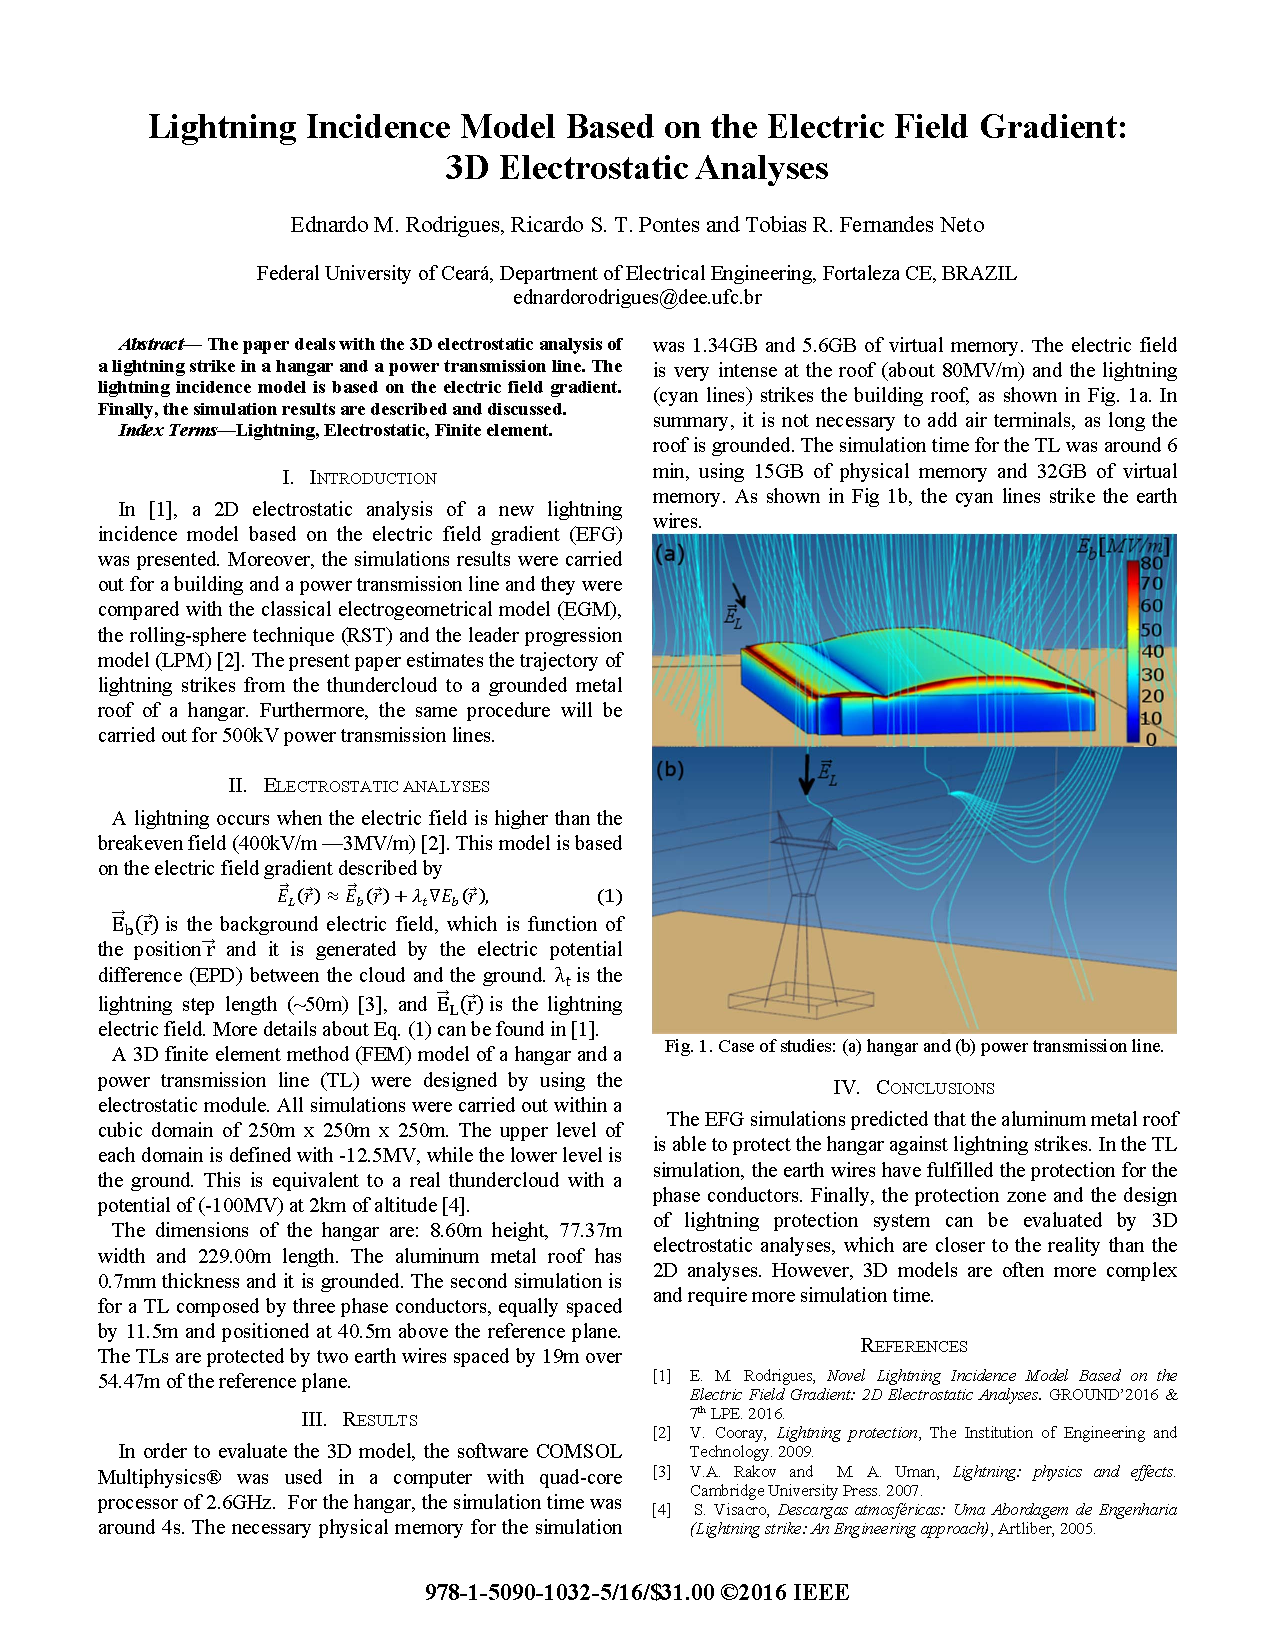
\includepdf[pages={-}]{3-pos-textuais/apendices/PID4416093.pdf}
	\imprimiranexos
		% Adicione aqui os anexos do seu trabalho
		\anexo{Exemplo de um anexo}
\label{an:ex_anexo_a}

Um anexo é um documento que não foi elaborado pelo autor, ou seja, o autor apenas anexa. Anexos podem ser tabelas, mapas, diagramas, \textit{datasheets}, manuais e etc. 




		\anexo{Exemplo de um anexo em PDF}
\label{an:ex_anexo_b}

O autor pode anexar um \gls{PDF}, traduzido como formato portátil de documento. Veja o código fonte utilizado para anexar o arquivo ``Sikasil.pdf'' que foi colocado dentro da pasta ``anexos'' que por sua vez está dentro da pasta ``elementos-pos-textuais''. Tenha muita atenção na hora de especificar o local do arquivo. Recomenda-se não utilizar caracteres especiais para nomear pastas e, principalmente, arquivos. 

Pode-se fazer uma descrição sucinta do arquivo anexado.

%Comando para incluir um arquivo em PDF:
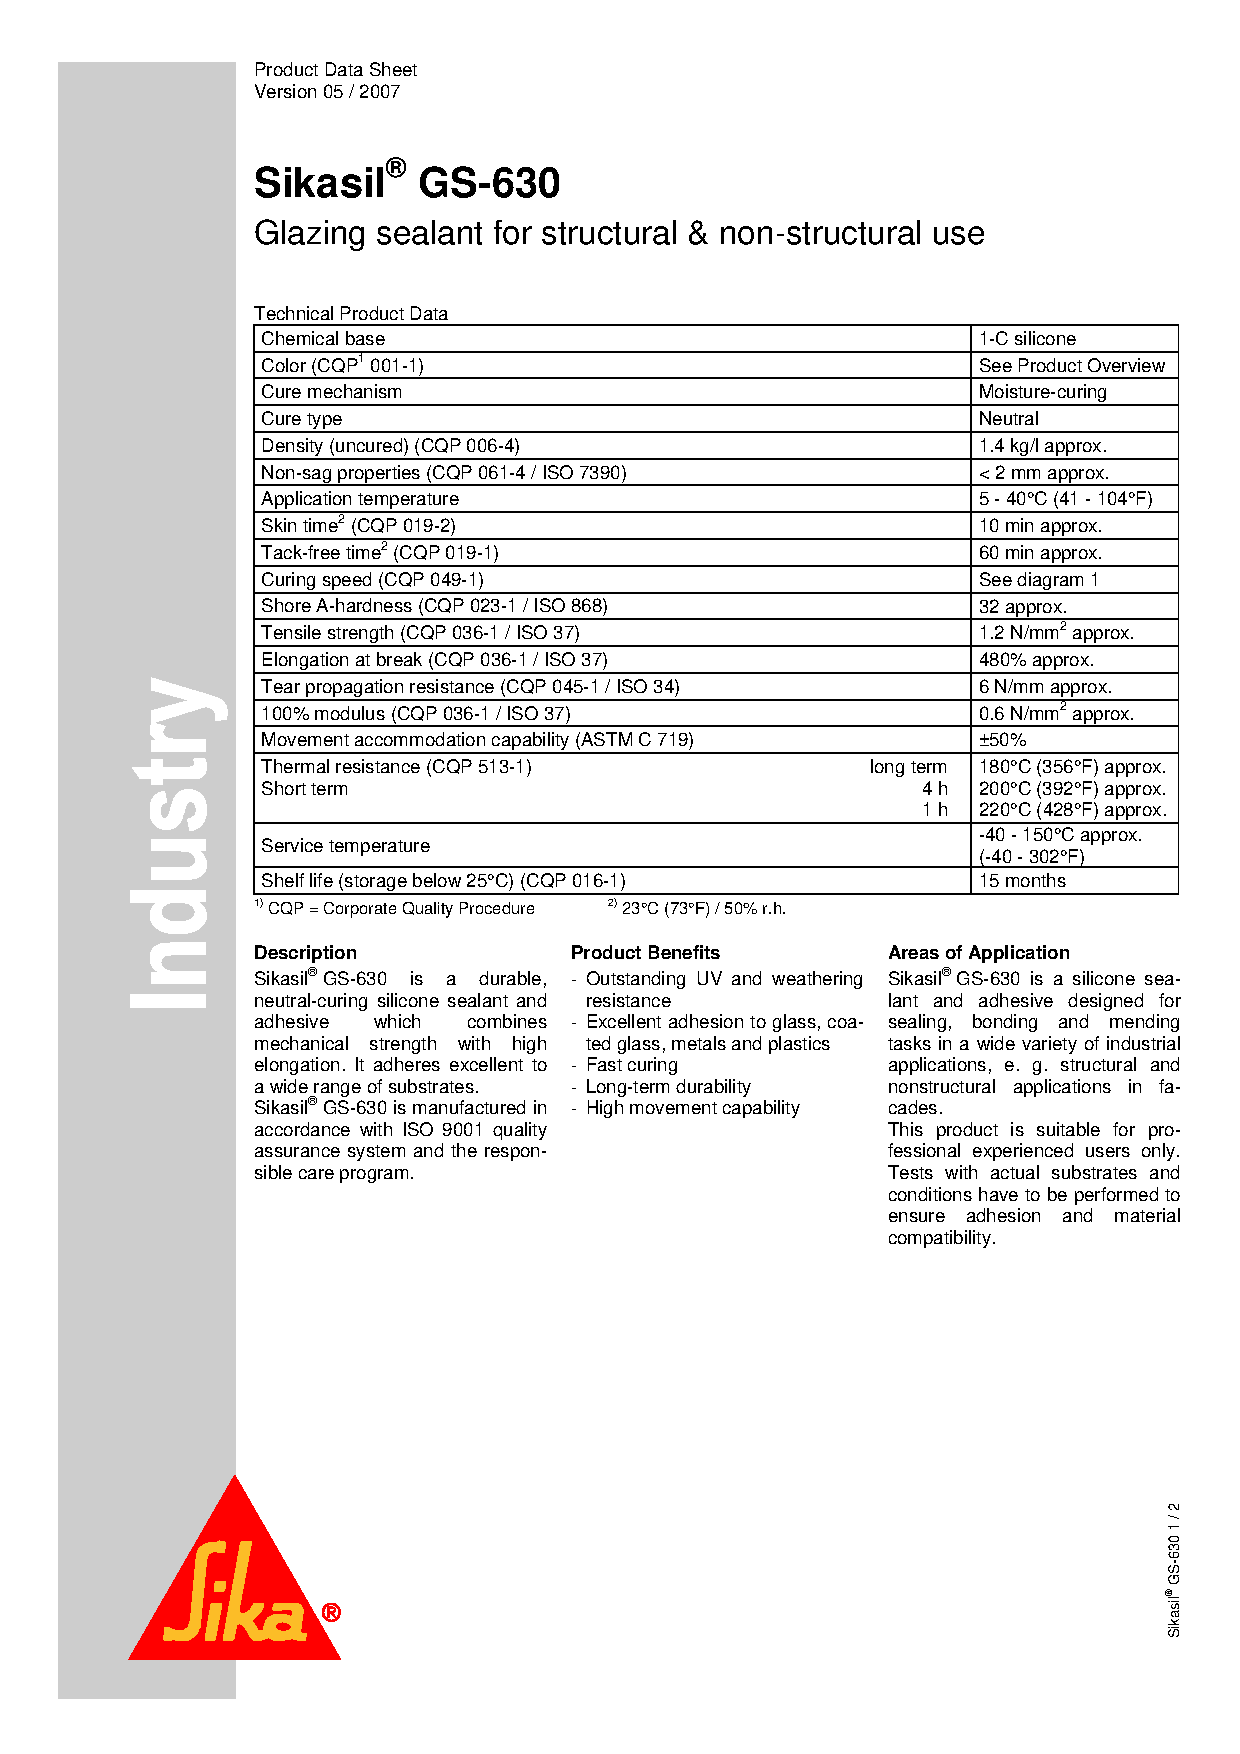
\includepdf[pages={-}]{3-pos-textuais/anexos/Sikasil.pdf}

		
    %\imprimirindice
    
	

\end{document}